\documentclass[a4paper, 11pt, titlepage]{article}
\usepackage{ucs}
\usepackage[german,ngerman]{babel}
\usepackage{fontenc}
\usepackage[pdftex]{graphicx}
\usepackage{listings}
\usepackage{xcolor}

\definecolor{codegreen}{rgb}{0,0.6,0}


\lstdefinestyle{mystyle}{  
    commentstyle=\color{codegreen},
    basicstyle=\ttfamily,
    breakatwhitespace=false,         
    breaklines=true,                 
    captionpos=b,                    
    keepspaces=true,                                    
    numbersep=5pt,                                 
    showstringspaces=false,
    showtabs=false,                  
    tabsize=2
}

\lstset{style=mystyle}

\renewcommand*{\thesubsection}{\alph{subsection}.}

\begin{document}
\title{Datenbanken \\
Ausarbeitung \"Ubung 6}

\author{Jakob Schulz}

\date{\today}

\maketitle{\thispagestyle{plain}}

\section{Aufgabe}
\subsection{}
SQL-Anweisung:
\begin{lstlisting}
select name
from titanic
where ticket = 'A/5. 3336'
\end{lstlisting}
Es handelt sich um ein Paar, welches die selbe Ticketnummer hat. Bei der Frau steht der gleiche Name wie beim Mann.
\subsection{}
Die Spalte sibsp zeigt an, wie viele Verwandte auf dem Schiff waren. Die Spalte parch gibt an, wie viele Kinder und Eltern eine Person hatte\\
SQL-Anweisung:
\begin{lstlisting}
select *
from titanic
where sibsp = 0 and parch = 0
\end{lstlisting}
\subsection{}
SQL-Anweisung:
\begin{lstlisting}
select distinct class
from titanic
\end{lstlisting}
Es gab die Klassen 1, 2 und 3.
\subsection{}
SQL-Anweisung:
\begin{lstlisting}
select name, fare, ticket
from titanic
where fare is null
\end{lstlisting}
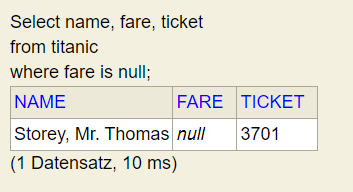
\includegraphics [width = 4 cm] {d}
\newpage
\subsection{}
SQL-Anweisung:
\begin{lstlisting}
select name, fare
from titanic
where fare = 0;
\end{lstlisting}
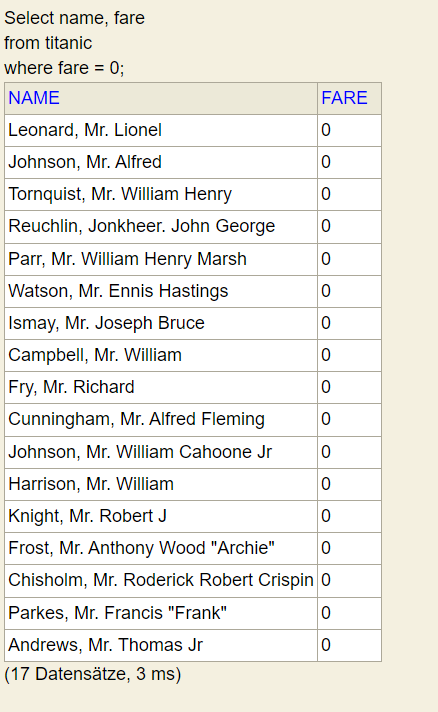
\includegraphics [width = 4 cm] {e}
\subsection{}
SQL-Anweisung:
\begin{lstlisting}
select ticket
from titanic
where name like '%Astor%'
\end{lstlisting}
John Jacob Astor ist mit dem Ticket "`PC 17757"' gereist.
\subsection{}
SQL-Anweisung:
\begin{lstlisting}
select *
from titanic
where ticket = 'PC 17757'
\end{lstlisting}
Es sind Person mit Astor gereist, die nicht mit ihm verwandt sind\\
\\
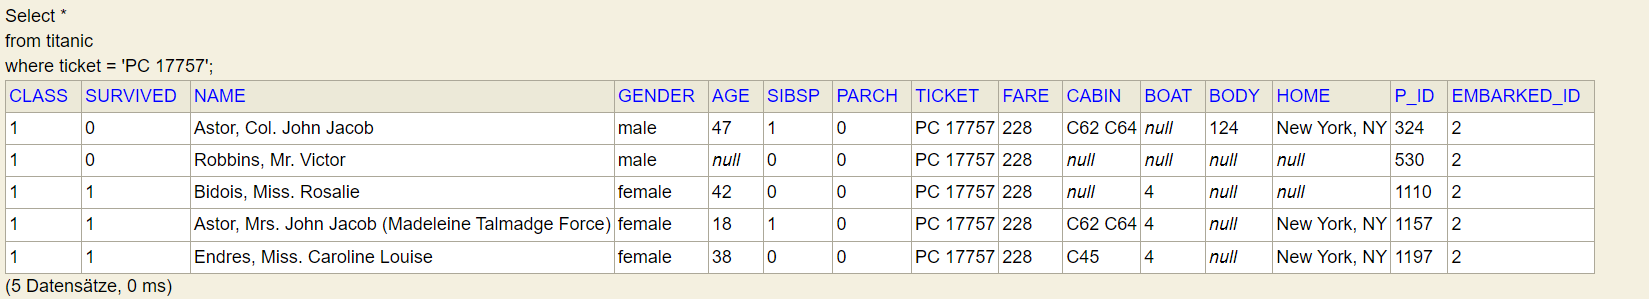
\includegraphics [width = 15 cm] {g}
\subsection{}
SQL-Anweisung:
\begin{lstlisting}
select name, boat, survived
from titanic
where boat is null and survived = 1
\end{lstlisting}
Es gibt Personen, die ohne Platz "uberlebt haben.
\subsection{}
SQL-Anweisung:
\begin{lstlisting}
select name, boat, survived
from titanic
where boat is not null and survived = 0
\end{lstlisting}
Ja, es gab Personen, die trotz einen Platz in einem Rettungsboot nicht überlebt haben\\
\\
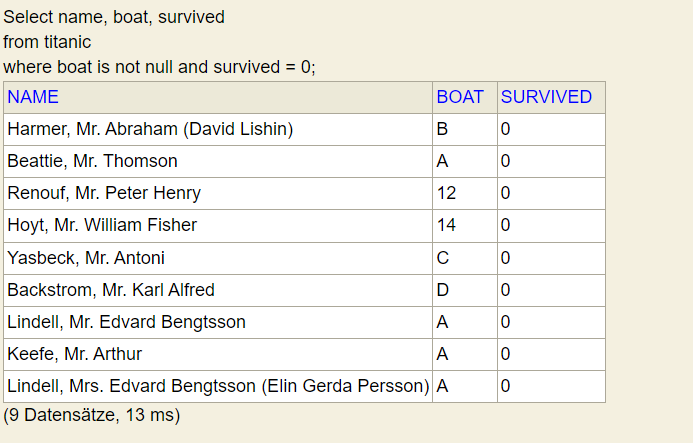
\includegraphics [width = 10 cm] {i}
\newpage
\subsection{}
SQL-Anweisung:
\begin{lstlisting}
select *
from titanic
where gender = 'male' and name not like '%Master%' 
and name not like '%Mr.%'
\end{lstlisting}
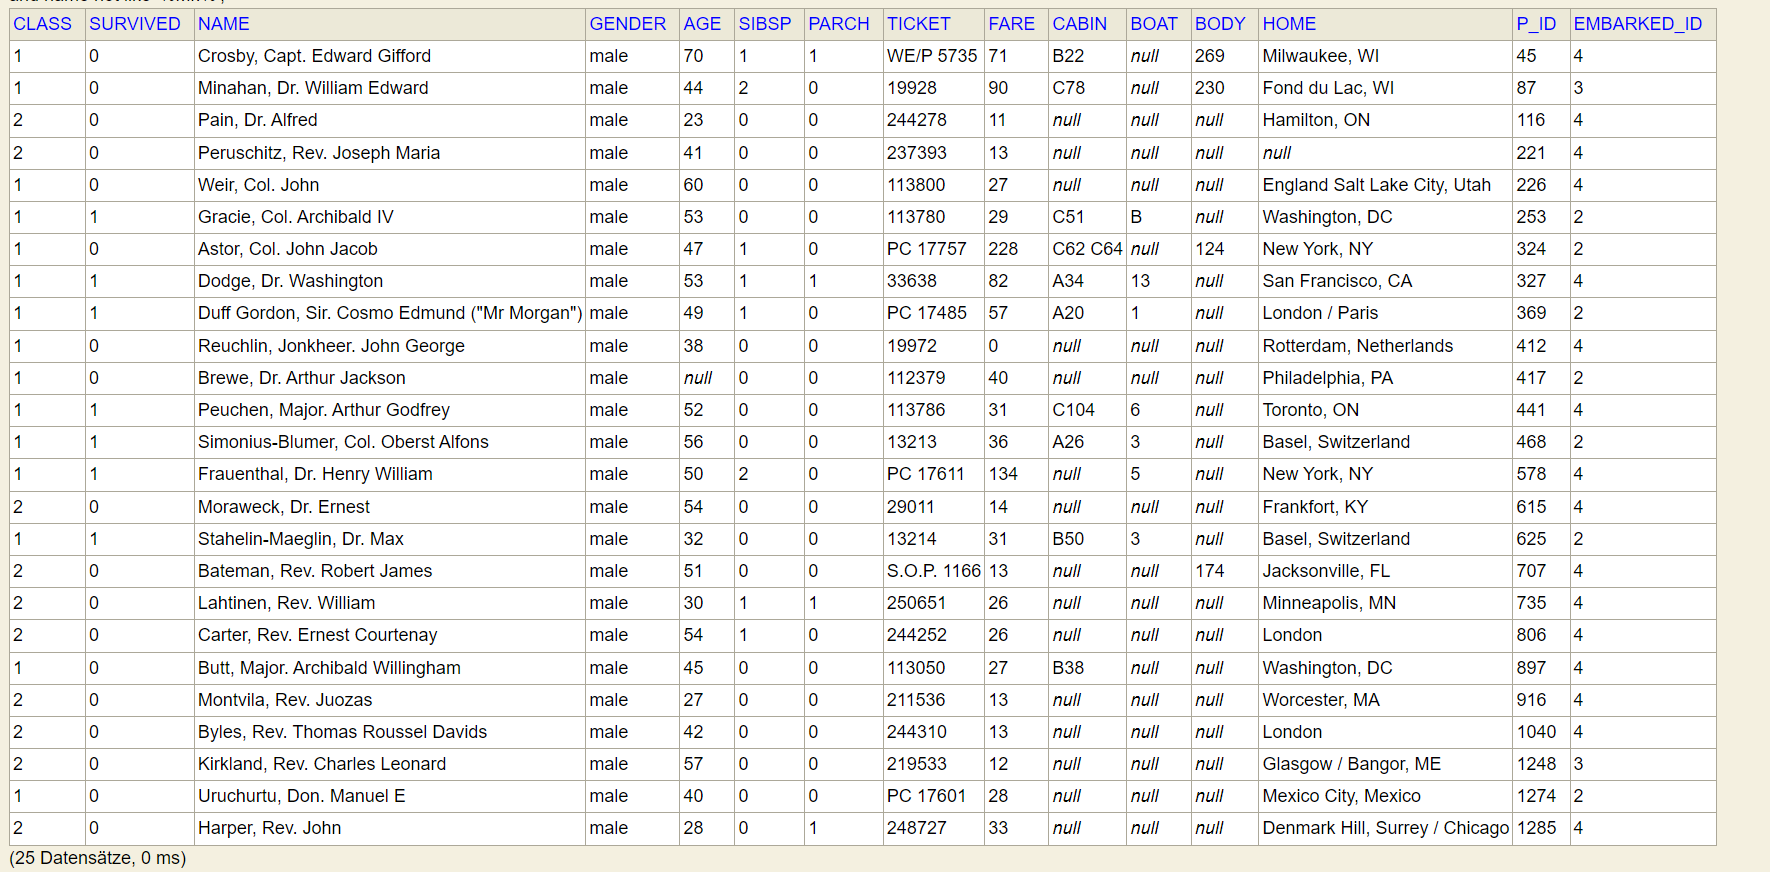
\includegraphics [width = 15 cm] {j}
\subsection{}
SQL-Anweisung:
\begin{lstlisting}
select distinct boat
from titanic
\end{lstlisting}
Man kann die Antwort nicht ohne weiteres ermitteln, weil mehrere Werte (Boote) in einer Zeile eingetragen sind. Vermutung: Man wusste bei manchen Personen nicht, in welchem Rettungsboot sie waren.\\
Man bekommt alle Zeilen mit nur einem Wert durch:\\
\begin{lstlisting}
select distinct boat
from titanic
where boat not like '% %'
\end{lstlisting}

\newpage
\subsection{}
SQL-Anweisung:
\begin{lstlisting}
select name, home
from titanic
where upper(home) like '%GERMANY%'
\end{lstlisting}
Ich habe hier upper verwendet, um zu vermeiden, dass kleine Schreibweisen nicht ausgegeben werden.\\
\\
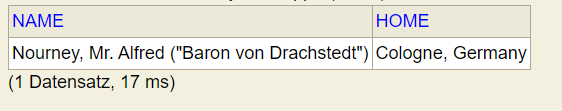
\includegraphics [width = 10 cm] {l}
\newpage
\subsection{}
SQL-Anweisung:
\begin{lstlisting}
select name, age, gender
from titanic
where age between 10 and 16 and gender = 'female'
\end{lstlisting}
Hier habe ich 10 und 16 als Grenzen verwendet, weil bei between die Grenzen auch noch ausgegeben werden.\\
\\
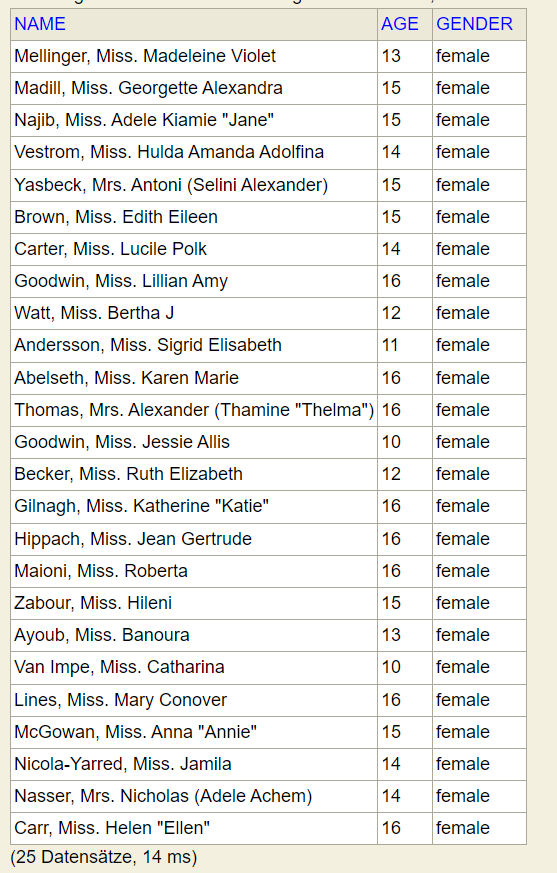
\includegraphics [width = 10 cm] {m}
\subsection{}
SQL-Anweisung:
\begin{lstlisting}
select name, age, sibsp
from titanic
where age <= 12 and sibsp = 0 and parch = 0;
\end{lstlisting}
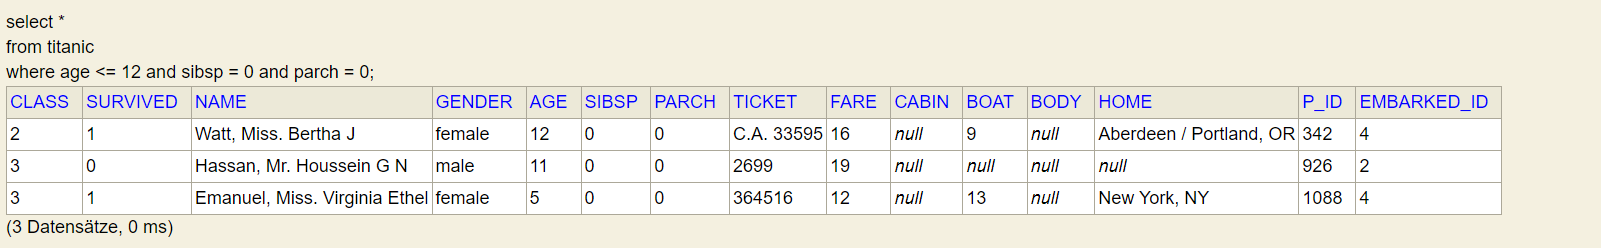
\includegraphics [width = 15 cm] {n}
\end{document}